% !TeX program = xelatex
% ============================================================
% 2026 年·北京卷数学（回忆版，内部候选） · 简答版
% 由 tools/make_editions.py 生成（重跑会覆盖本文件）；
% 题目/解析内容在 questions.tex / answers*.tex，勿在本文件内写内容。
% ============================================================
\documentclass[zihao=-4, a4paper]{ctexart}
% ============================================================
% common/preamble.tex —— 拆分版试卷项目 · 公共导言区
% 引擎：XeLaTeX；文档类 ctexart 由各版本壳文件自行声明
% 由合并书 math-gaokao-2017-2026/preamble.tex 改造而来：
%   - 页眉左右改为可重定义宏 \gkheadL / \gkheadR（各版本壳设置）
%   - hyperref 不再写死 pdftitle（壳内 \hypersetup 覆盖）
%   - 删除书籍专用的 \chaptermark 重定义与 \gkpaper 装配宏
% ============================================================

% ---------- 数学 ----------
\usepackage{amsmath}
\usepackage{amssymb}
\usepackage{mathtools}

% ---------- 绘图 ----------
\usepackage{tikz}
\usetikzlibrary{shapes.geometric, arrows.meta, calc, patterns, angles, quotes, positioning}
\usepackage{pgfplots}
\pgfplotsset{compat=1.18}

% ---------- 版面 ----------
\usepackage{geometry}
\usepackage{needspace}
\geometry{a4paper, margin=2.2cm, headheight=15pt}
% 紧凑版式（如印刷版）可在壳文件中于 \begin{document} 前再次调用 \geometry 覆盖
\usepackage{enumitem}
\setlist{itemsep=2pt, topsep=4pt, parsep=0pt}

% 中文与行内公式混排的断行弹性：
% emergencystretch 允许段落末路不通时追加伸展量；
% 降低二元/关系符罚分，允许行内长公式在 = 、+ 等处断行（否则整段外溢）
\emergencystretch=2em
\binoppenalty=700
\relpenalty=500
\usepackage{booktabs}      % 三线表
\usepackage[most]{tcolorbox}

% ---------- 选择题选项对齐 ----------
% tasks 宏包：\begin{gkopts}(列数) \task ... \end{gkopts}
% 自动等宽分栏，选项天然对齐；列数已由内容片段按选项长度写定（4/2/1）
\usepackage{tasks}
\settasks{label={}, label-width=0pt, item-indent=1.2em,
          column-sep=1em, after-item-skip=2pt, before-skip=2pt, after-skip=4pt}
\NewTasksEnvironment[style=itemize]{gkopts}[\task](4)

% ---------- 页眉页脚 ----------
\newcommand{\gkheadL}{}   % 左页眉：卷名（壳文件 \renewcommand 设置）
\newcommand{\gkheadR}{}   % 右页眉：版本名（壳文件 \renewcommand 设置）
\usepackage{fancyhdr}
\pagestyle{fancy}
\fancyhf{}
\fancyhead[L]{\small\gkheadL}
\fancyhead[R]{\small\gkheadR}
\fancyfoot[C]{\small —— 第 \thepage\ 页 ——}
\renewcommand{\headrulewidth}{0.4pt}

% ---------- 超链接（须最后加载）----------
\usepackage{hyperref}
\hypersetup{colorlinks=true, linkcolor=blue!55!black,
            bookmarksnumbered=true, unicode=true}

% ============================================================
% common/macros.tex —— 自定义命令与环境（题号、解析头、提示框等）
% 与合并书 math-gaokao-2017-2026/preamble.tex 的自定义段保持一致，
% 保证内容片段（questions.tex / answers.tex）在两个项目间可互换。
% ============================================================

% ---------- 试卷标识（壳文件 \renewcommand 设置，用于 label 命名空间）----------
\newcommand{\gkpaperid}{none}

% ---------- 题号 ----------
% 试题部分的题号：加粗编号 + 自动 \label{q:<卷id>:<题号>}
\newcommand{\gkti}[1]{\par\medskip\noindent
  \textbf{#1．}\phantomsection\label{q:\gkpaperid:#1}\ignorespaces}
% 多卷/分部重启题号时，#1 是唯一内部顺序号（交叉引用身份），#2 才是原卷显示题号。
\newcommand{\gktiwithlabel}[2]{\par\medskip\noindent
  \textbf{#2．}\phantomsection\label{q:\gkpaperid:#1}\ignorespaces}

% 解析部分的题头：小标题 + 回链到试题页
% （仅在题目与解析同文档的版本中回链有效；试题版不含解析头，无悬空引用）
\newcommand{\gksolhead}[2]{%
  \Needspace{3\baselineskip}\subsubsection*{第 #1 题\if\relax\detokenize{#2}\relax\else（#2）\fi}%
  \phantomsection\label{s:\gkpaperid:#1}%
  {\small\color{gray}（题目见第~\pageref{q:\gkpaperid:#1}~页）}\par\nopagebreak}
% 与 \gktiwithlabel 成对：显示原题号，但回链仍用唯一内部顺序号。
\newcommand{\gksolheadwithlabel}[3]{%
  \Needspace{3\baselineskip}\subsubsection*{第 #2 题\if\relax\detokenize{#3}\relax\else（#3）\fi}%
  \phantomsection\label{s:\gkpaperid:#1}%
  {\small\color{gray}（题目见第~\pageref{q:\gkpaperid:#1}~页）}\par\nopagebreak}

% ---------- 填空题空位 ----------
\newcommand{\gkblank}{\underline{\hspace{2.2em}}}

% ---------- 提示框 ----------
% 卷种提示 / 解析归属声明（醒目，浅黄）
\newtcolorbox{gknotice}{colback=yellow!8, colframe=orange!60!black,
  boxrule=0.5pt, arc=1.5pt, left=6pt, right=6pt, top=4pt, bottom=4pt,
  before skip=8pt, after skip=8pt}

% 方法提示 / 注（浅蓝，用于解析后的点评与题量说明）
\newtcolorbox{gktip}{colback=blue!4, colframe=blue!35!black,
  boxrule=0.4pt, arc=1.5pt, left=6pt, right=6pt, top=4pt, bottom=4pt,
  before skip=6pt, after skip=6pt, fontupper=\small}

% ---------- 答案行 ----------
% 解析中独立成段的"答案：X"用带底色的行呈现
\newcommand{\gkanswer}[1]{\par\smallskip\noindent
  \tcbox[width=\linewidth, tcbox width=auto limited,
         colback=green!6, colframe=green!35!black, boxrule=0.4pt,
         arc=1.5pt, left=4pt, right=4pt, top=2pt, bottom=2pt,
         nobeforeafter]{\textbf{#1}}\par\smallskip}

% ---------- 结构标题 ----------
% 结构标题后通常紧跟一个带 0.5\textheight 起始预留的解析题块；0.4 只够放标题，
% 会把下一题整体推到下一页，留下孤立的「二、填空题」等页尾标题。
\newcommand{\gkpart}[1]{\Needspace{0.6\textheight}\subsection*{#1}\nopagebreak}     % 标题 + 首题
% （一）必考题 / 解析小问标题：块式加粗段，可自动换行（\paragraph 的 run-in 版式会溢出）
\newcommand{\gksubpart}[1]{\Needspace{6\baselineskip}\par\medskip\noindent\textbf{#1}\par\nopagebreak\smallskip}

% 罗马数字Ⅰ-Ⅻ（U+2160）与圈号①②③（U+2460）划入 CJK 字符类，
% 用中文字体渲染——西文字体 Latin Modern 缺这些字形，否则整段静默丢字
\xeCJKDeclareCharClass{CJK}{"2160 -> "217F, "2460 -> "24FF}

% ============================================================
% common/questions_env.tex —— 题目 / 解析的语义包装环境
%
% questions.tex 中每道题包在 \begin{question}...\end{question} 里，
% answers.tex 中每题解析包在 \begin{answer}...\end{answer} 里；
% 题头排版仍由内容行中的 \gkti / \gksolhead 完成（见 macros.tex）。
%
% 环境本身不产生任何盒子或垂直间距（只引入一个 TeX 分组），
% 排版结果与不包裹时逐点一致。它的价值在于：
%   1. 给每道题一个机器可数的结构边界（校验脚本数环境数 = 题量）；
%   2. 为将来的条件编译留钩子——某版本可重定义环境实现按题取舍。
% ============================================================

% 环境不把整题装盒：题目与解析仍可自然跨页，但开始题块前必须为题面、
% 图形/表格或解析首段留出足够空间。仅保留 2 个 baseline 会让题干、
% 选项和图形在页边界处被拆开，形成不可打印的孤立内容；题目保留
% 0.15\textheight，在避免短题制造大段空白与避免题块拆分之间取平衡。
% 解析题块保留 0.5\textheight，以容纳“题面 + 图形/选项 + 首段解析”；
% 结构标题仍用更大的保留量；末页自然收尾由视觉复审判定。
\newenvironment{question}{\Needspace{0.15\textheight}}{}
\newenvironment{answer}{\Needspace{0.5\textheight}}{}

\renewcommand{\gkpaperid}{gk-2026-regular-beijing-recall}
\renewcommand{\gkheadL}{2026 年·北京卷数学（回忆版，内部候选） · 数学}
\renewcommand{\gkheadR}{简答版}
\hypersetup{pdftitle={2026 年·北京卷数学（回忆版，内部候选） 数学 · 简答版}}
\begin{document}
\begin{center}
  {\Large\bfseries 2026 年·北京卷数学（回忆版，内部候选）}\\[4pt]
  {\large 数学 · 简答版}
\end{center}
\medskip
\pdfbookmark[1]{试题}{sec:q}
% questions.tex —— 2026 年·北京卷数学（回忆版，内部候选） · 题目内容片段（无答案）
% 由 tools/generate_projects.py 依来源总账自 2026/2026_数学真题_北京回忆版_试题.md 生成，勿手改（改源 MD 后重跑）


\begin{gktip}
\textbf{来源说明}：本题面仅转录固定候选 PDF 的可见内容；固定 PDF 首页自称“回忆版”，发布者、版次、来源链及官方身份未认证。第三方异文报告链接：来源冲突复核。本稿不裁定哪个版本等同正式卷。
\end{gktip}

\gkpart{一、单选题}

\begin{question}
\gkti{1}\textbf{（源 PDF 第1页）} 

已知集合 \(M=\{x\mid -1<x<3\}\)，\(N=\{x\mid x\geq 2\}\)，则 \(M\cup N=\)（　）

\begin{itemize}
\item (A) \((2,3)\)
\item (B) \((-1,+\infty)\)
\item (C) \([2,3)\)
\item (D) \((-1,2]\)
\end{itemize}

\end{question}
\begin{question}
\gkti{2}\textbf{（源 PDF 第1页）} 

已知 \(z_1=3-2i\)，\(z_2=-1+4i\)，则 \(\lvert z_1+z_2\rvert=\)（　）

\begin{itemize}
\item (A) \(2\sqrt{2}\)
\item (B) \(i\)
\item (C) \(2\)
\item (D) \(8\)
\end{itemize}

\end{question}
\begin{question}
\gkti{3}\textbf{（源 PDF 第1页）} 

已知双曲线 \(C:\dfrac{x^2}{a^2}-\dfrac{y^2}{4}=1\ (a>0)\) 的渐近线方程为 \(y=\pm\dfrac{2}{3}x\)，则 \(a\) 的值为（　）

\begin{itemize}
\item (A) \(2\)
\item (B) \(3\)
\item (C) \(4\)
\item (D) \(9\)
\end{itemize}

\end{question}
\begin{question}
\gkti{4}\textbf{（源 PDF 第1页）} 

已知 \((a-\sqrt{x})^7\) 的展开式中的 \(x^2\) 的系数是 \(280\)，则 \(a=\)（　）

\begin{itemize}
\item (A) \(2\)
\item (B) \(-2\)
\item (C) \(1\)
\item (D) \(-1\)
\end{itemize}

\end{question}
\begin{question}
\gkti{5}\textbf{（源 PDF 第1页）} 

下列函数 \(f(x)\) 是奇函数且在定义域上单调递增的是（　）

\begin{itemize}
\item (A) \(f(x)=\dfrac{1}{x^2+1}\)
\item (B) \(f(x)=\sin x\)
\item (C) \(f(x)=2^{-x}-2^x\)
\item (D) \(f(x)=\ln\dfrac{5+x}{5-x}\)
\end{itemize}

\end{question}
\begin{question}
\gkti{6}\textbf{（源 PDF 第1页）} 

已知向量 \(\vec a,\ \vec b\) 满足 \(\lvert\vec a-\vec b\rvert=2\)，\(\vec a=(2,0)\)，则 \(\lvert\vec b\rvert\) 的最大值为（　）

\begin{itemize}
\item (A) \(1\)
\item (B) \(2\)
\item (C) \(3\)
\item (D) \(4\)
\end{itemize}

\end{question}
\begin{question}
\gkti{7}\textbf{（源 PDF 第1页）} 

\(\{a_n\}\)，\(\{b_n\}\) 是无穷数列，则“存在常数 \(M\)，使 \(a_n\leq M\leq b_n\ (n=1,2,3,\cdots)\)”是“\(a_n\leq b_n\ (n=1,2,3,\cdots)\)”的（　）

\begin{itemize}
\item (A) 充分不必要条件
\item (B) 必要不充分条件
\item (C) 充分必要条件
\item (D) 既不充分也不必要条件
\end{itemize}

\end{question}
\begin{question}
\gkti{8}\textbf{（源 PDF 第1页）} 

\(f(x)=\sin(x+\varphi)\ (0<\varphi<2\pi)\)，将 \(f(x)\) 向 \(x\) 轴正方向平移 \(3\varphi\) 个单位，得到的函数图像与 \(f(x)\) 图像关于 \(x\) 轴对称，则 \(\varphi\) 的取值个数为（　）

\begin{itemize}
\item (A) \(1\)
\item (B) \(2\)
\item (C) \(3\)
\item (D) \(4\)
\end{itemize}

\end{question}
\begingroup
\renewenvironment{question}{\Needspace{0.3\textheight}}{}
\begin{question}
\gkti{9}\textbf{（源 PDF 第1页）} 

学校组织高一、高二学生参观甲、乙两地博物馆，每位学生可自主选择一处前往．已知高一学生总人数多于高二学生总人数，前往甲地的全体学生总数多于前往乙地的全体学生总数，则（　）

\begin{itemize}
\item (A) 去甲地的高一学生人数多于去乙地的高一学生人数
\item (B) 去甲地的高一学生人数多于去乙地的高二学生人数
\item (C) 去甲地的高一学生人数不多于去乙地的高二学生人数
\item (D) 去乙地的高二学生人数不少于去甲地的高二学生人数
\end{itemize}

\Needspace{0.4\textheight}
\end{question}
\endgroup
\begin{question}
\gkti{10}\textbf{（源 PDF 第1–2页）} 

\begin{gktip}
【编者待核注】固定回忆版候选 PDF 的 Q10 选项忠实照录于下。第三方六页 PDF 的四个选项区间均有端点或区间异文；来源报告记录逐项差异，版本归属未核，不据此择定选项。
\end{gktip}

摇杆机械装置，如图，\(A\text{，}B\) 为定点，\(C\text{，}D\) 是动点，\(AD=1\text{，}CD=3\text{，}BC=\dfrac{5}{2}\text{，}AB=4\)，则 \(\cos\angle ABC\) 的取值范围（　）
\nopagebreak[4]
\begin{center}% Generator: hand-authored TikZ schematic traced from the fixed source-visible four-bar outline and circle; all proportions are illustrative.
% Source ID: src-96ac0e772a0483bbf7cf803b94b1a1d8d8e1d2ae16b936b196e6abc05d1251ee
% PDF SHA-256: 7e840dc5c259cf05138337178794a58b6593dc7f2bf0d693826489856da416e9
% PDF page 2; question 10.
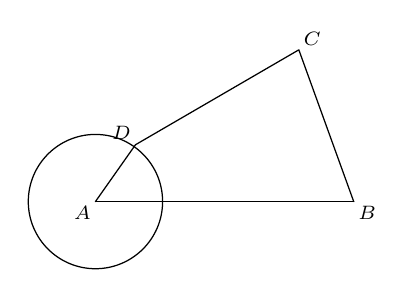
\begin{tikzpicture}[
  x=0.82cm,y=0.82cm,line width=0.45pt,line cap=round,line join=round,
  every node/.style={font=\scriptsize,inner sep=1.5pt}
]
  \coordinate (A) at (0,0);
  \coordinate (B) at (4,0);
  \coordinate (D) at (0.62,0.88);
  \coordinate (C) at (3.15,2.35);

  % The source shows a complete circle centered visually at A; it is not labelled as a trajectory.
  \draw (A) circle[radius=1.04];
  \draw (A)--(B);
  \draw (A)--(D)--(C)--(B);

  \node[below left] at (A) {$A$};
  \node[below right] at (B) {$B$};
  \node[above right] at (C) {$C$};
  \node[above left] at (D) {$D$};
\end{tikzpicture}
\end{center}
\nopagebreak[4]
\begin{itemize}
\item (A) \(\left[\dfrac{5}{16},\dfrac{53}{80}\right]\)
\item (B) \(\left[\dfrac{5}{16},\dfrac{73}{80}\right]\)
\item (C) \(\left[\dfrac{5}{12},\dfrac{53}{80}\right]\)
\item (D) \(\left[\dfrac{5}{12},\dfrac{73}{80}\right]\)
\end{itemize}

\end{question}
\gkpart{二、填空题}

\begin{question}
\gkti{11}\textbf{（源 PDF 第2页）} 

已知直线 \(ax+y=0\) 与圆 \((x-2)^2+(y-2)^2=4\) 相切，则 \(a=\underline{\qquad}\)。

\end{question}
\begin{question}
\gkti{12}\textbf{（源 PDF 第2页）} 

已知等差数列 \(\{a_n\}\) 的前 \(n\) 项和为 \(S_n\)，且 \(S_6=6a_6+30\)，则公差 \(d=\underline{\qquad}\)，若 \(S_n\leq S_5\) 恒成立，则符合条件的 \(a_1\) 的一个取值为\(\underline{\qquad}\)。

\end{question}
\begin{question}
\gkti{13}\textbf{（源 PDF 第2页）} 

\begin{gktip}
【编者待核注】固定回忆版候选 PDF 上限为 \(3\lg 2\)（含等号）；第三方 PDF 作严格小于。固定来源字面照录，端点异文未裁定。
\end{gktip}

音高 \(y\)（单位:mel）与频率 \(f\)（单位：Hz）满足 \(y=\lg\left(1+\dfrac{f}{700}\right)\)，若 \(\lg 2\leq y\leq 3\lg 2\)，则 \(f\) 的取值范围为\(\underline{\qquad}\)。

\Needspace{0.4\textheight}
\end{question}
\begin{question}
\gkti{14}\textbf{（源 PDF 第2页）} 

已知三棱锥 \(A-BCD\)，\(AD=AB=AC=2\sqrt{2}\)，\(BD=BC=2\)，\(DC=2\sqrt{3}\)，则它的底面 \(BCD\) 的面积为\(\underline{\qquad}\)，体积为\(\underline{\qquad}\)。
\nopagebreak[4]
\begin{center}% Generator: hand-authored TikZ schematic traced from the fixed source-visible tetrahedron edges; projection is illustrative.
% Source ID: src-96ac0e772a0483bbf7cf803b94b1a1d8d8e1d2ae16b936b196e6abc05d1251ee
% PDF SHA-256: 7e840dc5c259cf05138337178794a58b6593dc7f2bf0d693826489856da416e9
% PDF page 2; question 14.
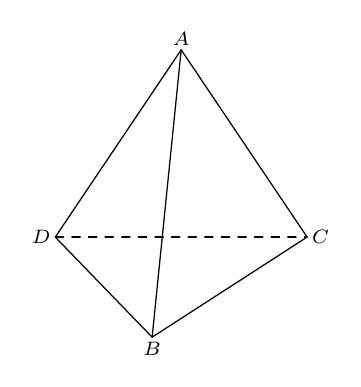
\begin{tikzpicture}[
  x=0.82cm,y=0.82cm,line width=0.45pt,line cap=round,line join=round,
  every node/.style={font=\scriptsize,inner sep=1.5pt}
]
  \coordinate (A) at (0,2.9);
  \coordinate (D) at (-1.95,0);
  \coordinate (C) at (1.95,0);
  \coordinate (B) at (-0.45,-1.55);

  % DC is the only hidden edge in the source.
  \draw[dashed] (D)--(C);
  \draw (A)--(D)--(B)--(C)--(A);
  \draw (A)--(B);

  \node[above] at (A) {$A$};
  \node[left] at (D) {$D$};
  \node[right] at (C) {$C$};
  \node[below] at (B) {$B$};
\end{tikzpicture}
\end{center}
\nopagebreak[4]
\end{question}
\begin{question}
\gkti{15}\textbf{（源 PDF 第2页）} 

\begin{gktip}
【编者待核注】固定回忆版候选 PDF 将“\(c=1\)”列为②、“\(c=0\)”列为③；第三方 PDF 交换这两个序号。两版来源链均不足以认证正式卷字面。
\end{gktip}

已知 \(f(x)=\lvert x^2-\cos x-c^2\rvert\)，给出下列四个结论：

① \(f(x)\) 在 \((-1,1]\) 上有最小值和最大值；

② \(c=1,\ x\in(-1,2]\) 时，\(f(x)\) 有最大值；

③ \(c=0,\ f(x)=1\) 有3个解；

④ \(c>0,\ f(x)\) 与 \(y=c\) 有4个交点。

其中正确结论的序号是\(\underline{\qquad}\)。

\end{question}
\gkpart{三、解答题}

\begin{question}
\gkti{16}\textbf{（源 PDF 第2页）} 

已知函数 \(f(x)=2\sin\omega x\cos\varphi+2\cos\omega x\sin\varphi\)，\(\omega>0,\ \lvert\varphi\rvert<\dfrac{\pi}{2}\)。\(f(x)\) 最小正周期为 \(\pi\)，且 \(f(0)>0,\ f\left(\dfrac{\pi}{4}\right)=1\)。

(1) 求 \(\omega\text{、}\varphi\) 的值；

(2) 求 \(f(x)\) 的单调递减区间。

\end{question}
\begin{question}
\gkti{17}\textbf{（源 PDF 第3页）} 

现从全校学生中随机抽取200人统计数学成绩，成绩分组及对应人数如下：

\begin{center}
\begin{tabular}{lrrrrr}
\toprule
成绩分组 & \([81,94)\) & \([94,107)\) & \([107,120)\) & \([120,135)\) & \([135,150]\) \\
\midrule
人数 & 40 & 60 & 60 & 32 & 8 \\
\bottomrule
\end{tabular}
\end{center}

以频率估计概率，完成下列问题：

(1) 求数学成绩低于120分的概率；

(2) 从学校随机抽取4人，求2人不低于120且2人小于94的概率；

(3) 每组数据取左端、中间、右端，比较 \(s_{\text{左}}^2\text{、}s_{\text{中}}^2\text{、}s_{\text{右}}^2\) 的大小关系。

\Needspace{0.4\textheight}
\end{question}
\begin{question}
\gkti{18}\textbf{（源 PDF 第3页）} 

已知直三棱柱 \(ABC-A_1B_1C_1\)，\(\angle BAC=90^\circ\)，\(AB=AC=2\)，\(BB_1=\sqrt{2}\)，\(E\text{、}D\) 分别为 \(A_1B_1\text{、}AC\) 的中点。
\nopagebreak[4]
\begin{center}% Generator: hand-authored TikZ schematic traced from the fixed source-visible prism edges and auxiliary lines; projection is illustrative.
% Source ID: src-96ac0e772a0483bbf7cf803b94b1a1d8d8e1d2ae16b936b196e6abc05d1251ee
% PDF SHA-256: 7e840dc5c259cf05138337178794a58b6593dc7f2bf0d693826489856da416e9
% PDF page 3; question 18.
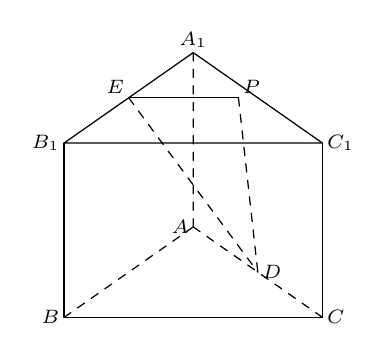
\begin{tikzpicture}[
  x=0.82cm,y=0.82cm,line width=0.45pt,line cap=round,line join=round,
  every node/.style={font=\scriptsize,inner sep=1.5pt}
]
  \coordinate (A)  at (0,-0.2);
  \coordinate (B)  at (-2,-1.6);
  \coordinate (C)  at (2,-1.6);
  \coordinate (A1) at (0,2.5);
  \coordinate (B1) at (-2,1.1);
  \coordinate (C1) at (2,1.1);
  \coordinate (E)  at (-1,1.8);
  \coordinate (D)  at (1,-0.9);
  \coordinate (P)  at (0.7,1.8);

  % Hidden prism edges from the source.
  \draw[dashed] (A)--(B) (A)--(C) (A)--(A1);

  % Auxiliary lines: EP is solid; ED and PD are dashed in the source.
  \draw[dashed] (E)--(D) (P)--(D);
  \draw (E)--(P);

  % Visible prism edges.
  \draw (B)--(C) (B)--(B1) (C)--(C1);
  \draw (A1)--(B1)--(C1)--cycle;

  \node[above] at (A1) {$A_1$};
  \node[left] at (B1) {$B_1$};
  \node[right] at (C1) {$C_1$};
  \node[left] at (B) {$B$};
  \node[right] at (C) {$C$};
  \node[left] at (A) {$A$};
  \node[above left] at (E) {$E$};
  \node[above right] at (P) {$P$};
  \node[right] at (D) {$D$};
\end{tikzpicture}
\end{center}
\nopagebreak[4]
(1) 证明：\(DE\parallel\)平面 \(BB_1C_1C\)；

(2) 点 \(P\) 在平面 \(A_1B_1C_1\) 内，且 \(EP\parallel B_1C_1\)，再从条件①、条件②、条件③这三个条件中选择一个作为已知，使得 \(P\) 唯一确定，求平面 \(PAD\) 与平面 \(PDE\) 的夹角的余弦值。

① \(PA=PD\)；

② \(PA\perp BC\)；

③ \(BB_1\parallel\)平面 \(PDE\)。

注：如果选择条件①、条件②、条件③分别解答，按第一个解答计分。

\end{question}
\begin{question}
\gkti{19}\textbf{（源 PDF 第4页）} 

已知椭圆 \(E:\dfrac{x^2}{a^2}+\dfrac{y^2}{b^2}=1\ (a>b>0)\) 的一个顶点是 \((2,0)\)，离心率为 \(\dfrac{1}{2}\)。

(1) 求 \(E\) 的方程；

(2) 过点 \(A(1,1)\)，斜率为 \(k\ (k\ne\pm1)\) 的直线交椭圆 \(E\) 于 \(B\text{、}C\) 两点，\(B\) 关于 \(y=x\) 的对称点为 \(D\)，\(DC\) 交 \(y=x\) 于 \(Q\)，若 \(\left\lvert S_{\triangle ABQ}-S_{\triangle ACQ}\right\rvert=\dfrac{5}{8}\)，求 \(k\)。

\end{question}
\begin{question}
\gkti{20}\textbf{（源 PDF 第4页）} 

设函数 \(f(x)=x^2+mx-4e^{nx-1}\ (n\in\mathbb{Z})\)，曲线 \(y=f(x)\) 在点 \((-1,f(-1))\) 处的切线方程为 \(4x+e^2y+e^2+8=0\)。

(1) 求 \(m\text{，}n\) 的值；

(2) 求 \(f(x)\) 的极值点个数；

(3) 求 \(y=kx-1\ (k>0)\) 与 \(f(x)\) 交点个数。

\end{question}
\begin{question}
\gkti{21}\textbf{（源 PDF 第5页）} 

设 \(A=(a_{ij})_{m\times n}\) 是一个 \(m\) 行 \(n\) 列的数阵，且数阵中的每一项 \(a_{ij}\in\{-1,1\}\)，都等于1或$-$1。若对任意 \(1\leq i,p\leq m,\ 1\leq j,q\leq n\)，其中 \(i\ne p,\ j\ne q\)，且 \(\bigl\lvert\lvert i-p\rvert-\lvert j-q\rvert\bigr\rvert=2\)，都有 \(a_{ij}+a_{iq}+a_{pj}+a_{pq}=0\)，则称数阵 \(A\) 具有性质 \(P\)。

\Needspace{5\baselineskip}
(1) 判断下列两个数表是否具有性质 \(P\)。

\nopagebreak[4]
\[
A_1=
\begin{pmatrix}
1&1&-1&1\\
-1&1&-1&1
\end{pmatrix},
\qquad
A_2=
\begin{pmatrix}
1&1&-1&-1\\
1&-1&1&-1\\
-1&1&-1&1
\end{pmatrix}.
\]

(2) 若 \(m=5,\ n=4\)，则具有性质 \(P\) 的数阵 \(A\) 中1的个数最多是多少？

(3) 若 \(m=n=6,\ a_{11}=1\)，且数阵 \(A\) 具有性质 \(P\)，证明：对任意 \(i\text{，}j\in\{1,2,3,4,5,6\}\)，都有 \(a_{ij}=a_{i1}a_{1j}\)。

\end{question}
\clearpage
\pdfbookmark[1]{答案速查}{sec:a}
\Needspace{8\baselineskip}
\begin{center}{\Large\bfseries 答案速查}\end{center}
\medskip
% answers_short.tex —— 2026 年·北京卷数学（回忆版，内部候选） · 简短答案速查
% 由 tools/make_short_answers.py 自 answers.tex 的 \gksolhead/\gkanswer 提取，
% 并与 2026/2026_数学真题_北京回忆版_答案要点.md 逐题比对后生成，勿手改（改源 MD 后重跑）。

\begin{gknotice}
\textbf{使用说明}：本节只给最终答案便于快速核对，完整推导见解析版。答案为编写者独立推导，\textbf{非官方标准答案}。
\end{gknotice}

\begin{gknotice}
选择题答案中的 U 表示待核，未给出猜测答案，详情见解析版。
\end{gknotice}

\gkpart{单选题}
\begin{center}\begin{tabular}{ccccccccccc}
\toprule
题号 & 1 & 2 & 3 & 4 & 5 & 6 & 7 & 8 & 9 & 10 \\
\midrule
答案 & B & A & B & A & D & D & A & C & B & U \\
\bottomrule
\end{tabular}\end{center}

\gkpart{填空题}
\begin{itemize}[leftmargin=2.6em]
  \item[\textbf{11.}] \(0\)
  \item[\textbf{12.}] \(d=-2\)；\(a_1\in[8,10]\)，例如 \(a_1=8\)
  \item[\textbf{13.}] U/PENDING；固定回忆版候选为 \([700,4900]\)，第三方异文对应 \([700,4900)\)
  \item[\textbf{14.}] 底面积 \(\sqrt3\)，体积 \(\dfrac{2\sqrt3}{3}\)
  \item[\textbf{15.}] ①②③④（②、③的原文序号有异文；两版下四项均成立）
\end{itemize}

\gkpart{解答题}
\begin{itemize}[leftmargin=2.6em]
  \item[\textbf{16.}] (1) \(\omega=2,\ \varphi=\dfrac\pi3\)；(2) \(\left[\dfrac\pi{12}+k\pi,\dfrac{7\pi}{12}+k\pi\right]\)，\(k\in\mathbb{Z}\)
  \item[\textbf{17.}] (1) \(0.8\)；(2) 独立多项分布模型下 \(\dfrac6{625}\)；(3) \(s_{\text{左}}^2<s_{\text{中}}^2<s_{\text{右}}^2\)
  \item[\textbf{18.}] (1) 见解析版；(2) U/PENDING；若取条件①或②，夹角余弦均为 \(\dfrac23\)；条件③不能唯一确定 \(P\)
  \item[\textbf{19.}] (1) \(\dfrac{x^2}{4}+\dfrac{y^2}{3}=1\)；(2) \(k=\pm\dfrac{\sqrt2}{4}\)；\(k=-\dfrac34\) 时 \(Q\) 不存在
  \item[\textbf{20.}] (1) \(m=2,n=1\)；(2) 2 个极值点；(3) 1 个交点
  \item[\textbf{21.}] (1) \(A_1\) 否，\(A_2\) 是；(2) 最多 12 个 1；(3) \(a_{ij}=a_{i1}a_{1j}\)
\end{itemize}

\end{document}
